\chapter{Increasing ABM Integration}
\label{chap:land}

% The last chapter was about the agricultural land-use ABM
% This chapter is going to be about the land-cover transition ABM
% This model also uses deep reinforcement learning in order to train agents
% The goal of this model is to demonstrate the predictive accuracy of the model
% and to prove the viability of the methodology, that being,
% that adding learning to an ABM allows for more meaningful decision-making
% AND that the ABM part allows the learning to capture features that
% might be hard to model otherwise

The previous chapter demonstrated how an agent-based model can be
implemented with machine learning in order to induce a model of
individual behavior.
This chapter will go on to show how this kind of agent-based model
can be integrated with a land cover model in order to predict
land cover change.

\section{Methodology}
\label{sec:land_methods}

The methodology here expands on the methodology presented in 
Chapter~\ref{chap:farm}.
This model is also an agent-based model, but instead of
focusing primarily on training the decision-policy of agents in the model,
the focus is on the land cover change that results as a byproduct of the
behavior of the agents.

\subsection{Modeling Land Cover Change}
\label{subsec:land_methods_cover}

Within the model, land cover is represented as a grid of cells.
Each cell has a land cover category, an NLCD land cover class,
a land use, and an associated land parcel. See Table~\ref{tab:land_cells}.

\begin{table}
\centering
\caption{Land Cell Features}
\label{tab:land_cells}
\begin{tabular}{llll}
\hline
\hline
    Parameter & Values \\
    \hline 
    Land Cover Category & Agricultural, Forested, Urban, Other \\
    NLCD Cover Class &  \\
    Land Usage Type & Managed/In-Use, Adjacent, Unmanaged \\
    \hline
\end{tabular}
\end{table}

Land cover change is modeled as a stochastic byproduct of agent
decision-making.
For example,
an agricultural agent deciding to increase its productivity
with regard to grazing animals may result in clearing forested land cells
and transitioning them to pasture.

These land-cover transitions 

Agent behavior is trained according to internal incentive structures,
the model and was trained on the validation accuracy of transitions
between land cover types in the validation dataset.

\begin{table}
\centering
\caption{Land Cover Categories}
\begin{tabular}{llc}
\hline
\hline
    Cover Category & NLCD Cover Class & Encoding \\
\hline
    Urban & Open Space Urban & 21 \\
    & Low Density Urban & 22 \\
    & Medium Density Urban & 23 \\
    & High Density Urban & 24 \\
    Forested & Deciduous Forest & 41 \\
    & Evergreen Forest & 42 \\
    & Mixed Forest & 43 \\
    Agricultural 
    & Pasture & 81 \\
    & Crops & 82\\
    Barren & Barren & 31 \\
    Grassland/Scrub & Scrub & 52 \\
    & Grassland & 71 \\
    Other & Water & 11 \\
    & Wetlands Woody & 90 \\
    & Wetlands Other & 95 \\
\hline
\end{tabular}
\end{table}

\textbf{Details}

%\subsection{Agent Networks and Connectivity}
%\label{subsec:land_methods_networking}

\section{Experimental Design}
\label{sec:land_exp}

\subsection{The Model}
\label{subsec:land_exp_model}

Real world land cover datasets for years: 2006, 2011, 2016.
Real world land cover transitions between 2006 and 2011 were
used as training and validation data for the land cover model.
Real world land cover transitions between 2011 and 2016 were
used as test data for the land cover model.

The real world transitions mapped from cover $A$ to cover $B$,
which is referred to as $\Delta_{A,B}$.
The modeled transitions for a parameterization $M(...)$ from cover $A$
to cover $\hat{B}$ is referred to as $\Delta_{A,\hat{B}}M(...)$.

\textbf{Explain meaning}

\subsubsection{Agents}
\label{subsubsec:land_exp_agents}

There are four types of agent present in this model:
agricultural agents,
forestry agents,
commercial agents, and
residential agents.

Agricultural agents model the behavior of farmers, herders, and other kinds of 
agricultural land managers within the study area.
They make annual decisions about their farming practices,
including whether they should change production in one of the four modeled 
agricultural industries (beef, dairy, corn, and hay) 
and whether they should implement an agricultural best management practice 
(BMP) to reduce phosphorous runoff on their land.
This agent type is very similar to how it was implemented in the
previous model; although, now, its productivity decisions can change
the land cover of the model.

Forester agents model the behavior of loggers and other kinds of
forested land managers within the study area.
They make annual decisions about their practices
and whether to implement an advised management practice (AMP).

Commercial agents model the behavior of shops, factories, offices, 
and other kinds of commercial land-holders within each study area. 
They make decisions trimonthly about their workforce, 
including their available jobs and the associated salaries
Byproducts of their actions impact the density and sprawl of urban
land cover on the landscape.

Residential agents model the behavior of renters and landowners within 
each study area. 
They make two decisions annually: whether to attempt a job change and whether 
to try to move house. 
Household satisfaction is valued as a combination of financial stability and 
mental satisfaction. 
Each household earns wages provided by a commercial agent --- 
these wages are determined by a stochastic process and can be adjusted by the 
job over time.
The decisions of these agents do not directly impact land cover change
on their associated parcel, but land cover can transition within their
parcel as a result of the decisions of other agents.

Agricultural and forestry agents are connected to and share information with
their $n$-nearest neighbors of the same agent type; these
networks are static throughout each model run.
Commercial and residential agents exist in a bipartite network with
one another.
This network is initialized via a stochastic process and is
updated as agents make decisions.

The learning architecture for agents of each type is
listed in Table~\ref{tab:land_anns}.

\begin{table}
\centering
\caption{Network parameters for the ANNs used by agents in each class
    for the land cover model}
\label{tab:land_anns}
    \begin{tabular}{@{\extracolsep{4pt}}lp{.05\linewidth}>{\centering}p{.05\linewidth}>{\centering}p{.05\linewidth}>{\centering}p{.05\linewidth}>{\centering}p{.05\linewidth}>{\centering}p{.05\linewidth}>{\centering}p{.05\linewidth}cc@{}}
\hline
\hline
\multirow{2}{*}{Parameter} 
    & \multicolumn{2}{c}{Agricultural} & \multicolumn{2}{c}{Forestry} 
    & \multicolumn{2}{c}{Commercial} & \multicolumn{2}{c}{Residential} \\
    \cline{2-3}\cline{4-5}\cline{6-7}\cline{8-9}
 & $\mu$ & $Q$ & $\mu$ & $Q$ & $\mu$ & $Q$ & $\mu$ & $Q$  \\
\hline
Input Nodes  & 15 & 32 & 10 & 15 & 4 & 10 & 5 & 9 \\
Inner Layers  & 4 & 3 & 4 & 3 & 2 & 2 & 2 & 2 \\
Inner Nodes  & 10 & 16 & 7 & 7 & 5 & 5 & 4 & 5 \\
Output Nodes  & 17 & 1 & 5 & 1 & 6 & 1 & 4 & 1 \\
\hline
\end{tabular}
\end{table}

\subsubsection{Execution Overview}
\label{subsubsec:land_exp_exe}

\textbf{Add Textual description of model execution and the timing of
model subsystems. Agents make decisions, then act and interact, then learn.}

\begin{figure}
\centering
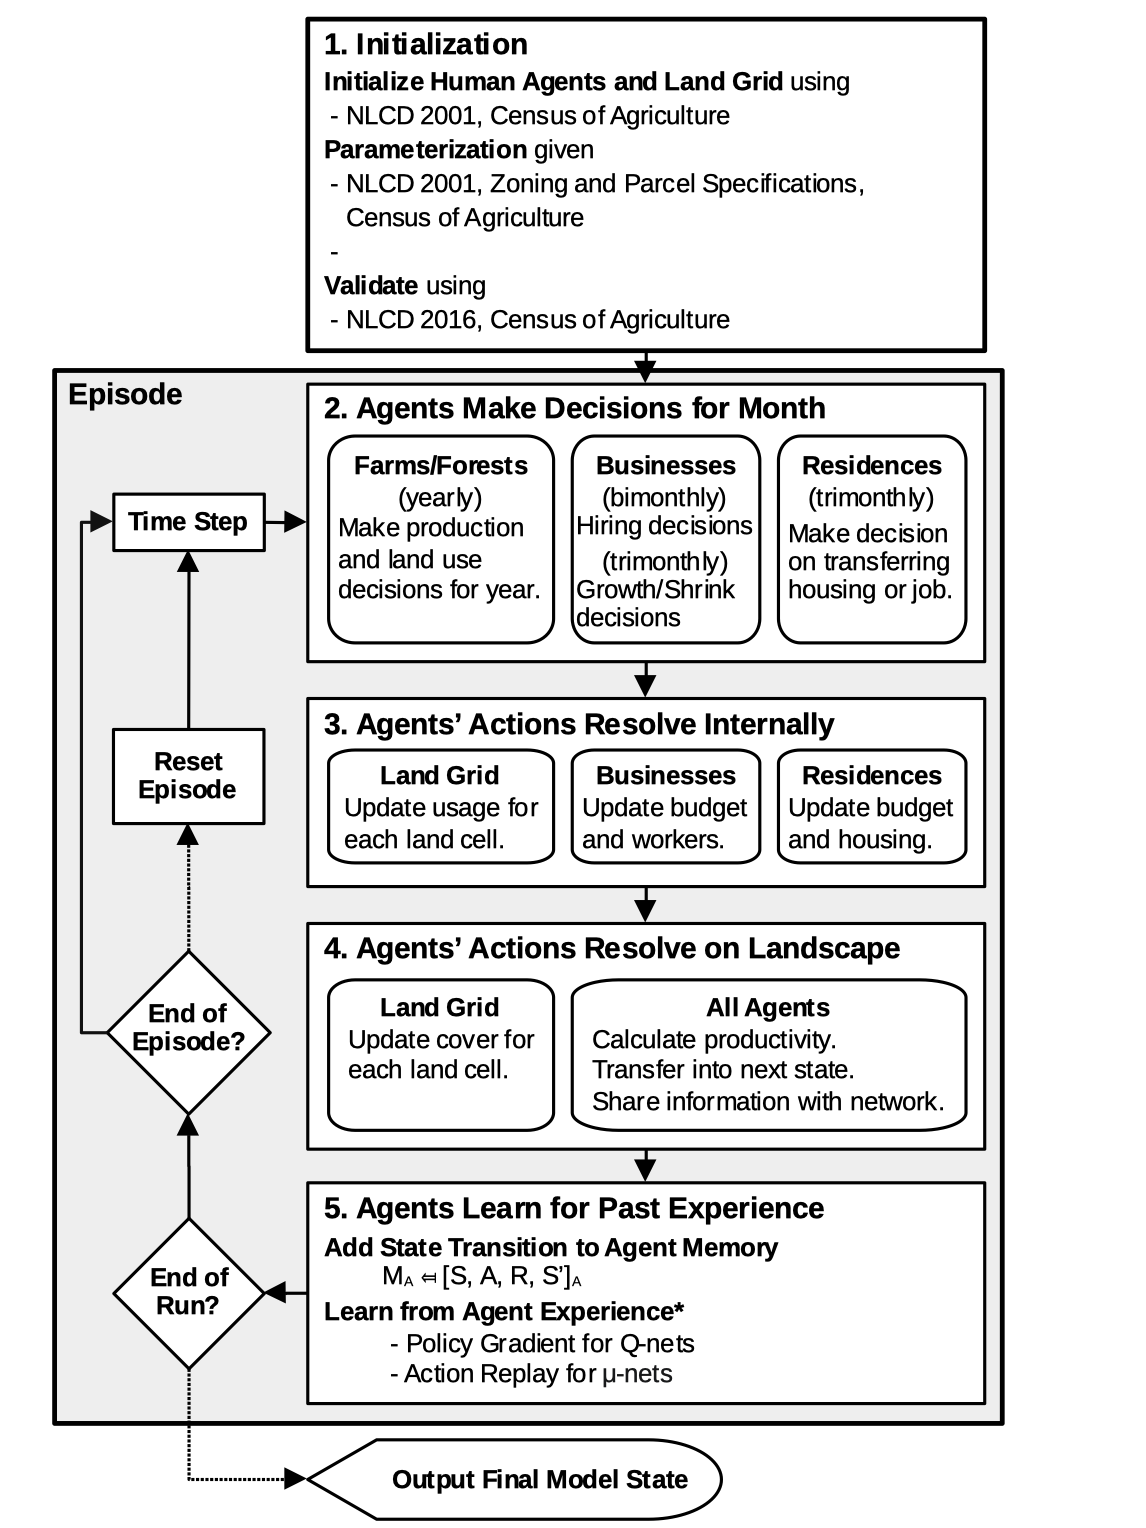
\includegraphics[width=0.7\textwidth]{figure/flowchart1.png}
\caption{Flowchart demonstrating the overall execution of the agent-based model
    and its coupling with the machine learning process}
\end{figure}

\subsection{Hyperparameter Selection}
\label{subsec:land_exp_hyper}

A summary of model hyperparameters is listed in Table~\ref{tab:land_hyper}.

\subsection{Experimental Setup}
\label{subsec:land_exp_setup}

Parameters were varied for experimental scenarios.

\textbf{Explain why this is more of a hyperparameter analysis. Because
we want to explore how agent interactivity and agent decision-making can
have secondary effects.}

\textbf{Include other parameters, or simple version?}

\begin{table}
\caption{Experimental parameters for the land cover transition model}
\centering
\begin{tabular}{ll}
\hline
\hline
    Variable & Values \\
    \hline
    Batch Size ($B$) & 8, 16, 32, 64 \\
    Discount Factor ($\gamma$) & 0.5, 0.9, 0.99 \\
%    Population Mixing ($P$) & 0.0, 0.25, 0.5, 0.75 \\
    Recall Accuracy ($F'$) & 0.0, 0.25, 0.5, 0.75 \\
    \hline
\end{tabular}
\end{table}

% As a second measure of model performance, a convolutional neural network (CNN)
% was trained on the same data as the agent-based model.
% The CNN was trained to predict the land cover of a cell at time $t_e$
% based on the land cover of the cell and it's surrounding neighborhood
% at time $t_s$.
% 
%     \^{C}=CNN(A)
% 
%     $\hat{C}=ConvNet(A)$
% 
% Parameters for the comparative CNN model.
% 
% \begin{table}
% \centering
%     \caption{Network architecture of comparative CNN}
%     \label{tab:land_cnn}
%     \begin{tabular}{lcccc}
%         \hline
%         \hline
%         Layer & Size & Stride & Kernel & Activation \\
%         \hline
%         Input & $5\times 5$ & 1 & --- & --- \\
%         Convolutional & $5\times 5$ & 1 & 6 & ReLU \\
%         Pooling & $2\times 2$ & 2 & --- & --- \\
%         Convolutional & $5\times 5$ & 1 & 16 & ReLU \\
%         Pooling & $2\times 2$ & 2 & --- & --- \\
%         Fully Connected & 120 & --- & --- & ReLU \\
%         Fully Connected & 84 & --- & --- & ReLU \\
%         Output & 17 & --- & --- & Softmax \\
%         \hline
%     \end{tabular}
% \end{table}

\subsection{Known Limitations}
\label{sec:land_lim}

Some types of land-cover transition either do not exist in the training
data or are not well-represented.
These types of transitions are rare within the study area,

\textbf{move and elaborate}

% For the purposes of analyzing the results of this model,
% where these types of transitions occur,
% they are treated as neither a successful nor an unsuccessful measure
% of model performance.
% Instead, they are treated as a separate neutral measure.
% 
% This limitation of the model is discussed in greater detail
% in Section~\ref{sec:land_disc}.
% 
% 
% For many of these missing transitions,
% there is a lack of any substantive literature supporting a predictive model 
% that is generalizable enough to meaningfully incorporate into the ABM.


\section{Results}
\label{sec:land_results}

\subsection{Model Performance}
\label{subsec:land_results_performance}

Model performance under each experimental parameterization was
evaluated by comparing the land cover in model year 2016 to
the recorded/observed land cover for the study area for real year 2016.

The Nash-Sutcliffe efficiency index (NSE) was used to evaluate
the goodness-of-fit of the model under each experimental parameterization.
The NSE is a measure of the relative magnitude of the residual variance
of modeled data compared to the residual variance of the observed data.
The value of the index ranges from $-\inf$ to $1$,
where a score of 1 indicates a perfect fit,
a score of 0 indicates that the model is no better than the mean of the
observed data,
and a score less than 0 indicates that the mean of the observed data
is a better predictor than the model.

This index was calculated in relation to three forms of model performance.
The first is the ability of the model to appropriately predict
the proportional coverage of each land cover type in the target year,
$\text{NSE}_\text{plc}$.
The second is the ability of the model to appropriately predict
the categorical transitions of land cover types from the start year to
the target year,
$\text{NSE}_\text{cat}$.
The third is the ability of the model to appropriately predict
the absolute transitions of land cover types from the start year to
the target year,
$\text{NSE}_\text{abs}$.
These indices are detailed below.

A majority of land cells in the study area do not transition land cover
between the start year and target year ($92.6\%, n=69124$),
which would heavily bias any analysis of model performance.
Therefore, the NSE was calculated only for those cells that transitioned
land cover.

The NSE measure of proportional coverage ($\text{NSE}_\text{plc}$),
shown in Equation~\ref{eq:nse_plc},
where $P_b$ represents the observed proportional coverage of land cover
type $b$ in the target year,
$\hat{P_b}$ represents the simulated proportional coverage of land cover
type $b$ in the target year,
and $\bar{P_b}$ represents the mean observed proportional coverage of
land cover type $b$ in the target year.

\begin{equation}
    \label{eq:nse_plc}
    \text{NSE}_{\text{plc}} 
    = \frac{\sum_b\left(P_b - \hat{P_b}\right)^2}
        {\sum_b\left(P_b-\bar{P_b}\right)^2}
\end{equation}

The NSE measure of categorical land cover transitions ($\text{NSE}_\text{cat}$),
shown in Equation~\ref{eq:nse_cat},
where $\Delta_{A,B}$ represents the number of observed transitions
from land cover category $A$ in the starting year to land cover
category $B$ in the target year,
where $\widehat{\Delta_{A,B}}$ represents the number of simulated transitions
from $A$ to $B$,
and where $\overline{\Delta_{A,B}}$ represents the mean observed number of
transitions from $A$ to $B$. \textbf{Not sure I'm saying this correctly.}

\begin{equation}
    \label{eq:nse_cat}
    \text{NSE}_{\text{cat}}
    = \frac{\sum_{A,B}\left(\Delta_{A,B}-\widehat{\Delta_{A,B}}\right)^2}
        {\sum_{A,B}\left(\Delta_{A,B}-\overline{\Delta_{A,B}}\right)^2},
    A \ne B
\end{equation}

The NSE measure for absolute land cover transition ($\text{NSE}_\text{act}$),
shown in Equation~\ref{eq:nse_act},
is very similar to the calculation of $\text{NSE}_\text{cat}$,
except that it is calculated for the absolute land cover class of each
land cell and not just its categorical class.
\textbf{NLCD Cover Class vs Coverage Category, f.x. for-deciduous vs forested}

\begin{equation}
    \label{eq:nse_act}
    \text{NSE}_{\text{abs}} 
    =
    \frac{\sum_{a,b}\left(\Delta_{a,b} - \widehat{\Delta_{a,b}}\right)^2}
        {\sum_{a,b}\left(\Delta_{a,b} - \overline{\Delta_{a,b}}\right)^2}
    ,
    a\ne b
\end{equation}

The maximum NSE values seen during testing runs were 
$\text{NSE}_\text{plc}=0.84$,
$\text{NSE}_\text{cat}=0.76$, and
$\text{NSE}_\text{act}=0.64$.

The sensitivity of NSE to each model parameterization across model
runs was evaluated by calculating the mean and variance of the NSE indices
under each parameterization. Figure~\ref{fig:land_nse}

\begin{figure}
    \centering
    \subcaptionbox{$\text{NSE}_\text{plc}$}{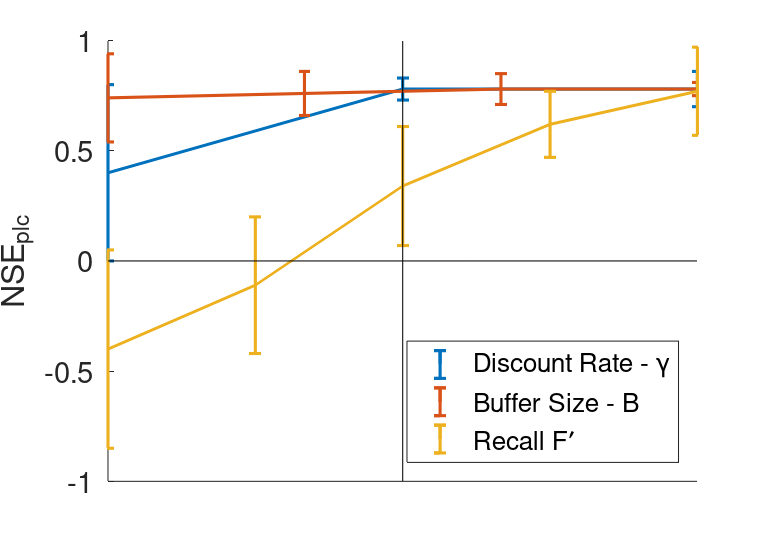
\includegraphics[width=0.3\textwidth]{figure/nscplc}}
    \hfill
    \subcaptionbox{$\text{NSE}_\text{cat}$}{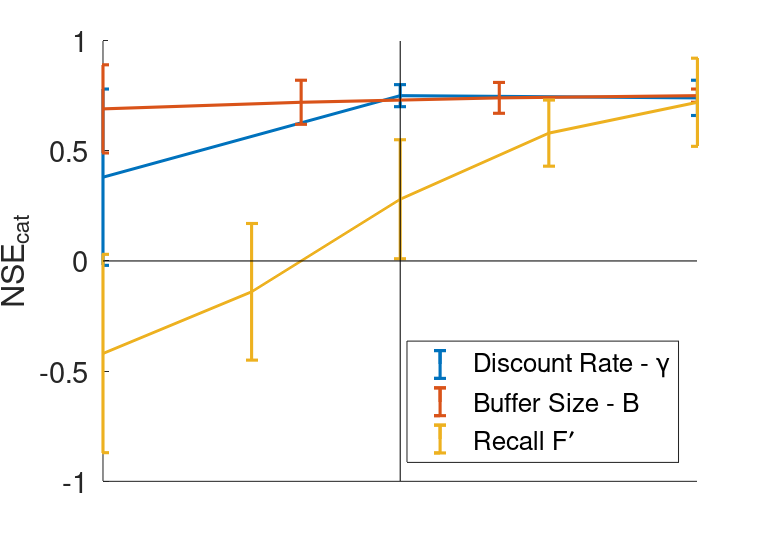
\includegraphics[width=0.3\textwidth]{figure/nsccat}}
    \hfill
    \subcaptionbox{$\text{NSE}_\text{act}$}{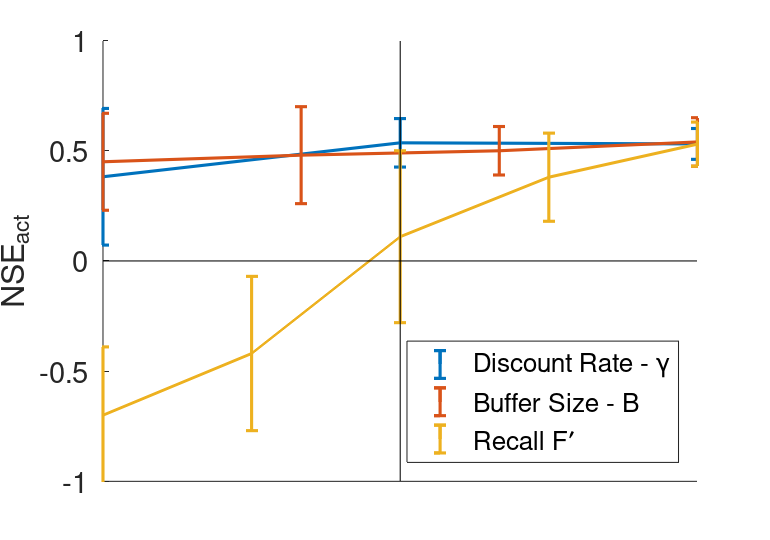
\includegraphics[width=0.3\textwidth]{figure/nscact}}
    \caption{NSE index sensity for each index showing the variance in
    model classification accuracy by each metric under different model
    parameterizations.}
    \label{fig:land_nse}
\end{figure}

\section{Discussion}
\label{sec:land_disc}

\textbf{Explain why it matters.}

\section{Agents}
\subsection{Agents}

Listing of agent state parameters.

\begin{table}
\begin{tabular}{llll}
\hline
\hline
    Name & Type & Range \\
    \hline
    Econ & float & -10 10 \\
\end{tabular}
\end{table}

